\section{Results}
In this section we let the Q-learning algorithm act on the the state spaces described in section \ref{sec:BMDP}. First, let $S_{hand}=\{  (s_{p1},\ldots,s_{p10},\Sigma_{d})\ s_{pi} \in \{1,2,\ldots, 21 \}, \Sigma_{d}\in \{1,2,\ldots, 10 \} \}$ and $S_{sum}=\{  (\Sigma_p, a_p, \Sigma_d )  \}$ denote the two state spaces. For abbreviation we may call these ''hand''- and ''sum''- environments or state spaces respectively. Also, we will simply call our Q-learning algorithm the ''algorithm''.

We will employ a $\eps$ greedy algorithm on the two state spaces where the values of the matrix $Q$ are initized to zero. The constant $\eps$ is chosen according to the algorithm and theory described in \ref{sec:impl}. The number of episodes is set to $10^7$ if not stated otherwise. 

%the sum space is a subset of the hand space we expect that the Q-learning perform better in cases when the decks are finite. 
%To ensure that the learning algorithm explores the state space we will use an $\eps$-greedy algorithm, if not stated otherwise. The decay of the $\eps$-greedy algorithm will be linear with the number of episodes has passed one tenth of the number of simulations. As an example, if we perform $10^6$ simulations then after a fixed point the proability of taking a random action will decay by $1 / \text{episode}$. Also, the initial values of $Q(S, a)$ will be zero for all states $S$ and actions $a$. 

In Figure \ref{fig:avg_return} we display the average return, by episodes, of the algorithm for different number of decks. The x-axis is scaled to a proportion of the number of simulations performed. In the top left Figure of Figure \ref{fig:avg_return}, denoted \ref{sfig:nd1}, we can see the performance of the Q-learning algorithm for 1 deck. Here, it becomes increasingly important to remember what cards that have been played. This is to be expected. When playing using one deck, there are only 4 of each card with the exception of all suites which are ten. Conditioned on the dealers outcome (where only one card is visible), the probability of seeing a arbitrary sequence of cards is relatively large for small deck sizes. However, as the deck size increases the information of what cards that are in your hand become redundant. This can be seen subsequently in Subfigures \ref{sfig:nd2}, \ref{sfig:nd8} and \ref{sfig:ndinf}. One could note that in subfigure \ref{sfig:nd2} of Figure \ref{fig:avg_return} the algorithm seem to have some reward left to accumulate. It has not yet converged. If more simulations were to be performed, the average reward of the hand might pass the sum's. 
\begin{figure}[htp]
\begin{tabular}{cc}
\centering
 \begin{subfigure}[b]{0.48\textwidth}
  	 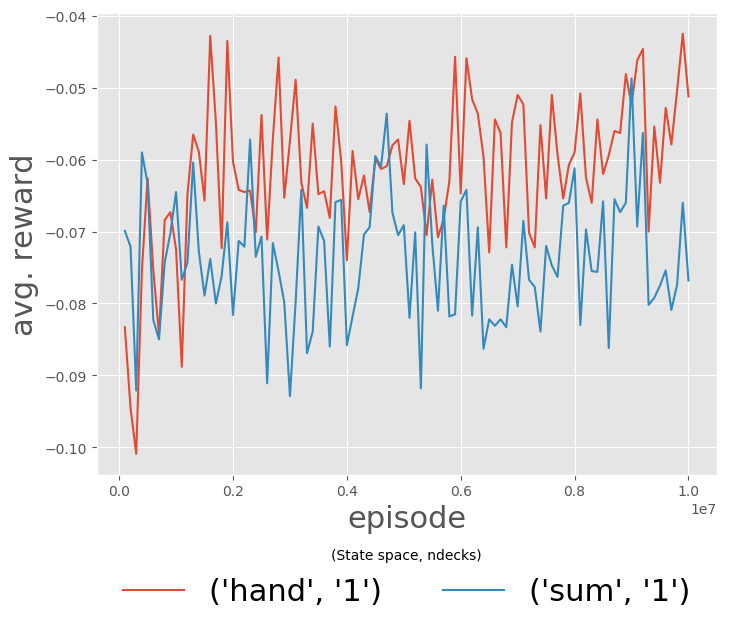
\includegraphics[width=\textwidth]{./figures/avgReturnEp_ndeck1.png}
   % .: 0x0 pixel, 0dpi, 0.00x0.00 cm, bb=
   \caption{Avg. return with 1 deck\label{sfig:nd1}}
 \end{subfigure}
 &
 \begin{subfigure}[b]{0.48\textwidth}
  	 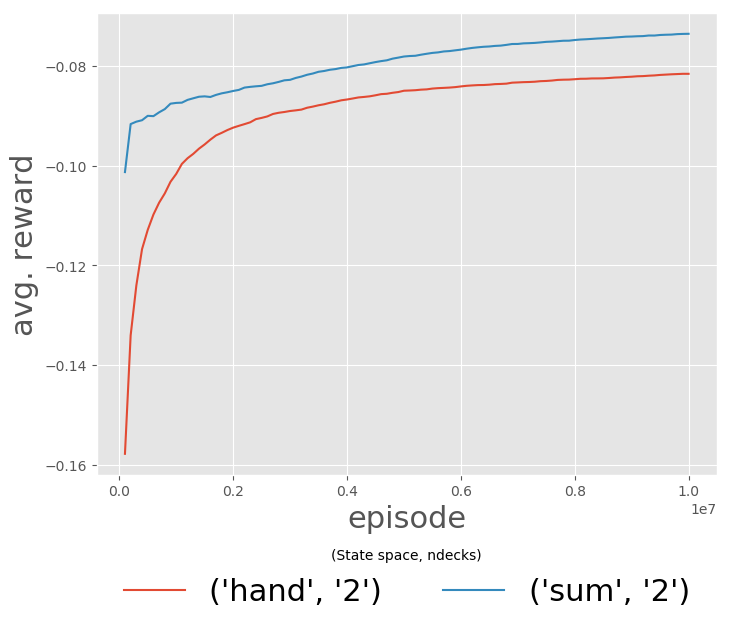
\includegraphics[width=\textwidth]{./figures/avgReturnEp_ndeck2.png}
   % .: 0x0 pixel, 0dpi, 0.00x0.00 cm, bb=
   \caption{Avg. return with 2 decks\label{sfig:nd2}}
 \end{subfigure}
 \\
 \begin{subfigure}[b]{0.48\textwidth}
  	 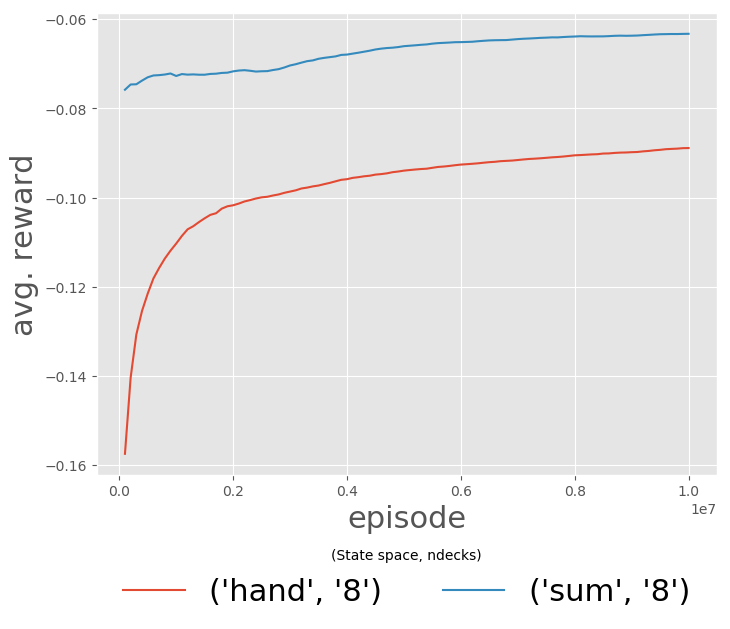
\includegraphics[width=\textwidth]{./figures/avgReturnEp_ndeck8.png}
   % .: 0x0 pixel, 0dpi, 0.00x0.00 cm, bb=
   \caption{Avg. return with 8 decks \label{sfig:nd8}}
 \end{subfigure}
 &
 \begin{subfigure}[b]{0.48\textwidth}
  	 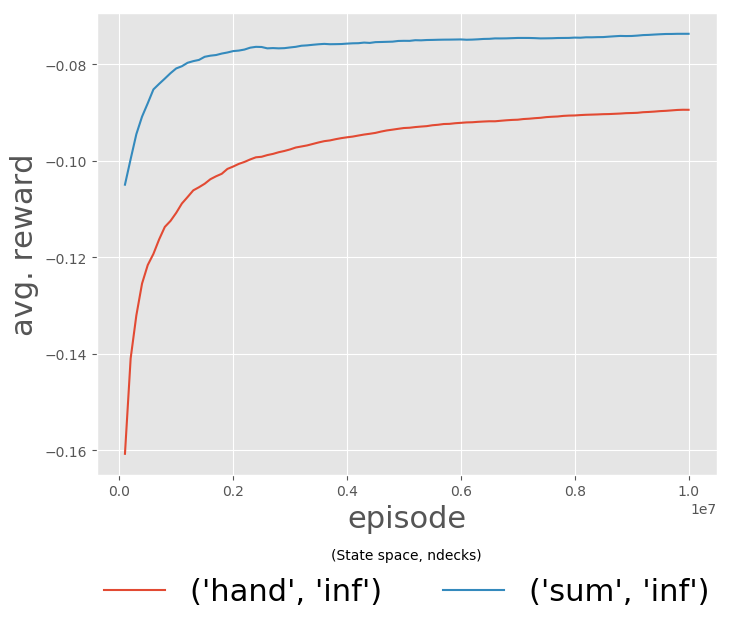
\includegraphics[width=\textwidth]{./figures/avgReturnEp_ndeckinf.png}
   % .: 0x0 pixel, 0dpi, 0.00x0.00 cm, bb=
   \caption{Avg. return with infinite decks \label{sfig:ndinf}}
 \end{subfigure}
\end{tabular}
\caption{The average return of an $\epsilon$-greedy Q-learning algorithm for TEST different state spaces. \label{fig:avg_return}}
\end{figure}

Since the cardinality of the hand space is much (!) larger then the sum's, the number of states the algorithm must explore will be larger. In Table \ref{tab:state_visited} we show the number of states the algorithm has explored together with the effective training time for the specific environment and the number of decks in play. We can clearly see that the number of explored grow increasingly large for the hand state when the number of decks increases. Interestingly, the number of explored states go stay around $70 000$ when having 8 decks and an infinite amount of decks. The number of states explored by the algorithm for the sum stays almost constant when increasing the number of decks.

Surprisingly, the training time for the hand state space is much larger than that of the sum space. By these results, there seem to be an indication that there is a $50\%$ increase in training time for the algorithm on the hand state compared to the sum. Note that the effective training time is simply the time it took to train this specific instance. It should only be interpreted as an indication of the time it takes to train one instance of the algorithm. All other measures of training time (which might be more accurate) are omitted because of the lack of computational power and time.
\begin{table}[h!]
\centering
 \begin{tabular}{c|cc|cc}
  \# decks & $\hat{S}_{hand}$ & $t_{hand}$ & $\hat{S}_{sum}$ &  $t_{sum}$  \\
  \hline 
  $1$ & $7693$ & $1423.286$ & $645$ & $940.998$ \\
  $2$ & $37671$ & $1520.298$ & $686$ & $1024.545$ \\
  $8$ & $70396$ & $1526.443$ & $680$ & $1023.590$ \\
  $\inf$ & $70756$ & $1515.659$ & $676$ & $1060.511$ 
 \end{tabular} 
 \caption{The number of explored states $\hat{S}$ and the training time $t$ (seconds) for a given number of decks in play and its respective state space. The number of simulations was set to $10^7$.\label{tab:state_visited}}
\end{table}

We are also interested in the 

\begin{figure}[htp]
\centering
 \begin{subfigure}[b]{0.48\textwidth}
  	 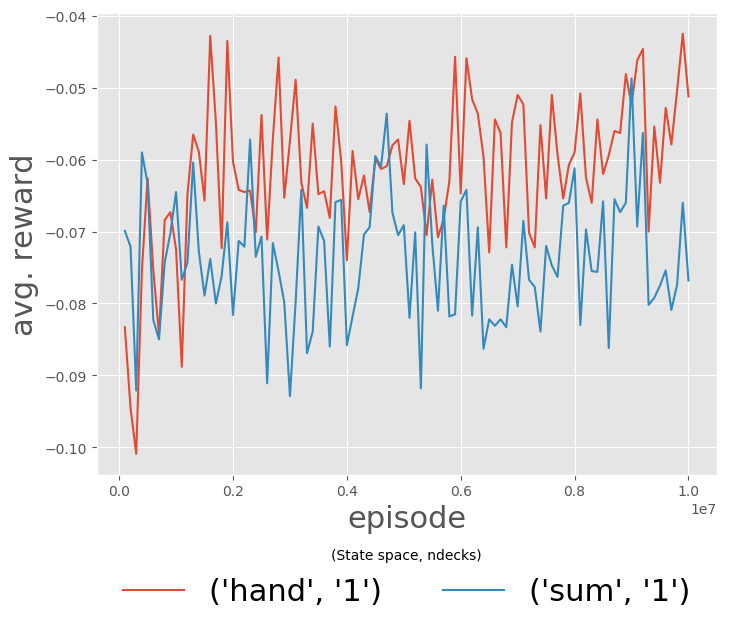
\includegraphics[width=\textwidth]{./figures/avgReturnEp_ndeck1.png}
   % .: 0x0 pixel, 0dpi, 0.00x0.00 cm, bb=
   \caption{Avg. return with 1 deck\label{sfig:3Dfignd6}}
 \end{subfigure}
 \begin{subfigure}[b]{0.48\textwidth}
  	 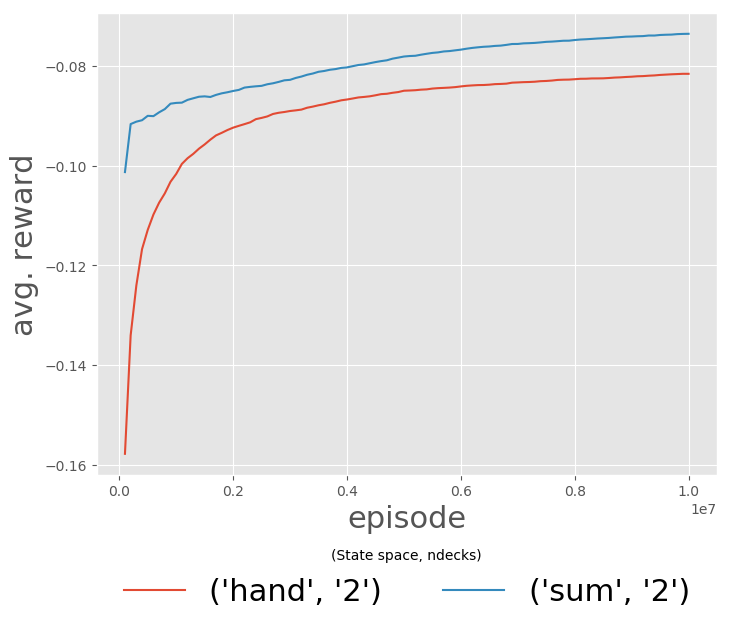
\includegraphics[width=\textwidth]{./figures/avgReturnEp_ndeck2.png}
   % .: 0x0 pixel, 0dpi, 0.00x0.00 cm, bb=
   \caption{Avg. return with 2 decks\label{sfig:3Dfignd8}}
 \end{subfigure}
\caption{The average return of an $\epsilon$-greedy Q-learning algorithm for TEST different state spaces. \label{fig:avg_return}}
\end{figure}